\chapter[~~~CONCEPTION]{~~~II -~Conception de l’application}%
\label{refDev2}%

Ce chapitre explique la conception de l'application \nom\~et les choix réalisés pour sa réalisation. Il détaille les diagrammes de classes, les structures de données et les algorithmes intéressants.

\section{Diagramme de classes}

Cette section présente le diagramme de classes du projet \nom. Il est composé de plusieurs classes et interfaces.
% \bigskip

\begin{figure}[!ht] 
  \centering% 
  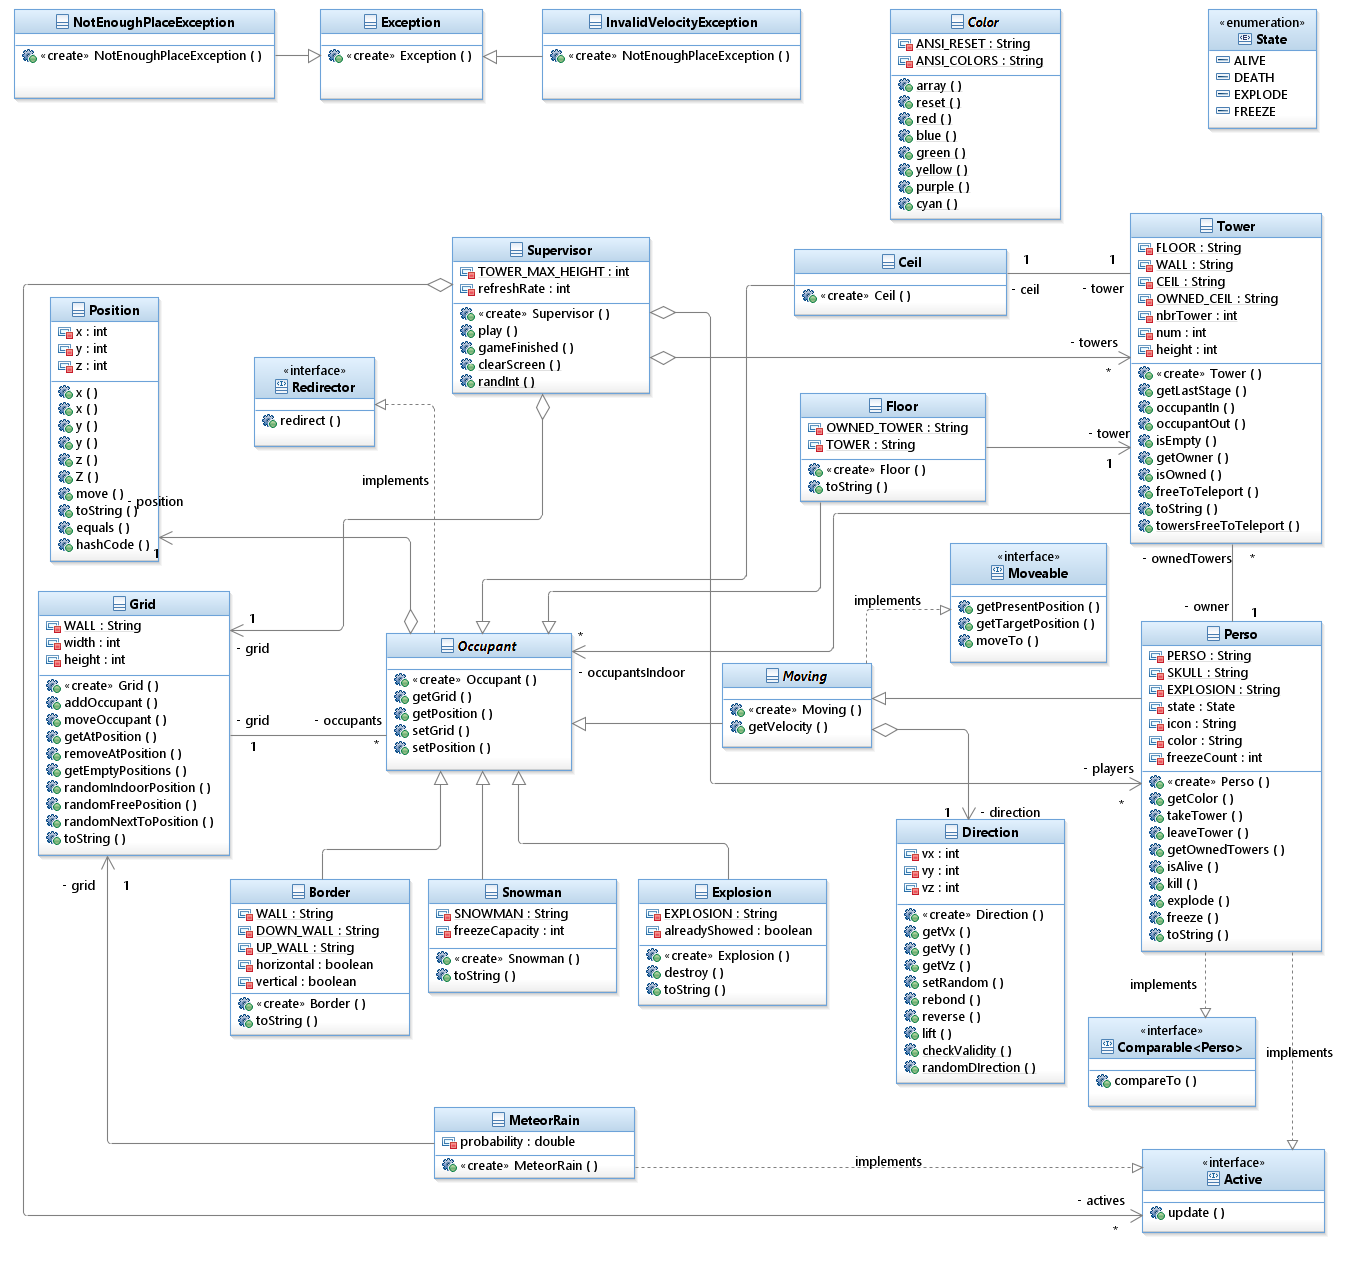
\includegraphics[width=13.9cm]{assets/pictures/ToursInfernales_Main.png} 
  \caption{Diagramme de classes complet du projet}%
  %\label{Q1}
\end{figure}
\newpage

\section{Choix des structures de données}

Le projet \nom\~utilise plusieurs structures de données pour stocker les informations des personnages, des murs et des tours:

\begin{itemize}
    \item \textcolor{cardinal}{structures de données}.
    \item \textcolor{cardinal}{structures de données}.
    \item \textcolor{cardinal}{structures de données}.
\end{itemize}

\section{Algorithmes intéressants}

\textcolor{cardinal}{Algorithmes intéressants}

%%% algo balise meta pour le non-indexage d'un site
% \begin{algorithm}
% \caption[\emph{Balise Meta pour le non-indexage d'un site}]{\label{non_indexage}Exemple d'une balise meta pour empêcher l'indexage d'un site à la ligne 7.}
% %\textbf{\textcolor{teal}{<!\,-\,- commentaire -\,->}}\\
% \textbf{<!\textcolor{blue}{DOCTYPE} \textcolor{cyan}{html}>}\\
% \html{}{
%   \head{}{
%   \smallskip
  
%     \textbf{<\textcolor{blue}{title}>Exemple de non-indexage</\textcolor{blue}{title}>\\
%     <\textcolor{blue}{meta} \textcolor{cyan}{charset}=\textcolor{auburn}{“UTF-8”}>\\
%     \dots\\
%     <\textcolor{blue}{meta} \textcolor{cyan}{name}=\textcolor{auburn}{“robots”} \textcolor{cyan}{content}=\textcolor{auburn}{“noindex”}>\\}
%     \smallskip
    
%   }
%   \smallskip
   
%   \body{}{
%   \smallskip
  
%   \dots\\
%   \smallskip
  
%   }
% }
% \end{algorithm}
\bigskip
